% 1977 年江苏卷第 3 题：直角三角形中的高与中线
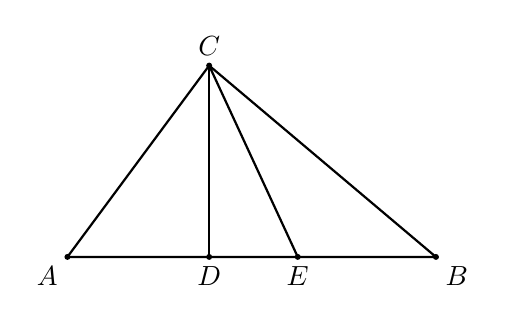
\begin{tikzpicture}[scale=0.9]
  \coordinate (A) at (0,0);
  \coordinate (D) at (2.0,0);
  \coordinate (E) at (3.25,0);
  \coordinate (B) at (5.2,0);
  \coordinate (C) at (2.0,2.7);
  \draw[thick] (A)--(C)--(B)--cycle;
  \draw[thick] (C)--(D);
  \draw[thick] (C)--(E);
  \fill (A) circle (1.2pt) node[below left] {$A$};
  \fill (B) circle (1.2pt) node[below right] {$B$};
  \fill (C) circle (1.2pt) node[above] {$C$};
  \fill (D) circle (1.2pt) node[below] {$D$};
  \fill (E) circle (1.2pt) node[below] {$E$};
\end{tikzpicture}
